\chapter{Controle hormonal da reprodução}\label{ch:b2:reproductive-hormones}

Todo mês, num calendário mantido com precisão de um ou dois dias
durante trinta anos, um \omterm{def:b2:mammal-reproduction:ovary}{folículo} amadurece, um óvulo é liberado, o
revestimento do útero é construído e depois, a menos que um embrião
tenha chegado, destruído. Nenhum relógio do corpo bate nesse ritmo; o
ritmo emerge de um diálogo entre três órgãos --- o hipotálamo, a
hipófise e o ovário ---, no qual cada hormônio controla a liberação do
seguinte e o último controla o primeiro. Este capítulo desmonta esse
diálogo: o eixo que comanda os dois sexos, o controle tônico do
\omterm{def:b2:mammal-reproduction:testis}{testículo}, o controle cíclico do ovário, com sua notável passagem da
retroalimentação negativa à positiva, e as maneiras como o eixo é
sobrepujado pela gestação, pelos fármacos e pela clínica.

\section{O eixo}

\begin{definition}[O eixo hipotálamo-hipófise-gônadas]\label{def:b2:reproductive-hormones:axis}
\index{hormônio liberador de gonadotrofinas}\index{hormônio luteinizante}\index{hormônio folículo-estimulante}\index{retroalimentação negativa!hormonal}
Neurônios do \emph{hipotálamo} secretam o \emph{GnRH} (hormônio
liberador de gonadotrofinas, um peptídeo de dez aminoácidos) nos
pequenos vasos porta que seguem até a \emph{adeno-hipófise}, em
breves \emph{pulsos} a cada uma ou duas horas. O GnRH faz a hipófise
secretar na circulação geral dois hormônios glicoproteicos, as
\emph{gonadotrofinas} \emph{LH} (hormônio luteinizante) e \emph{FSH}
(hormônio folículo-estimulante). Estas agem sobre as \emph{gônadas}: o
LH sobre as células produtoras de esteroides (\omterm{def:b2:mammal-reproduction:testis}{células de Leydig},
células da teca e células luteínicas), o FSH sobre as células que
nutrem os gametas (\omterm{def:b2:mammal-reproduction:testis}{células de Sertoli} e da granulosa). As gônadas
respondem com esteroides --- \emph{testosterona}, \emph{estradiol},
\emph{progesterona} --- e com o peptídeo \emph{inibina}, e estes
exercem retroalimentação sobre o hipotálamo e a hipófise: os
esteroides sobre ambos, sobretudo \emph{negativamente}; a inibina
apenas sobre o FSH. O resultado é uma alça regulada, na qual a
produção da gônada é mantida num valor de referência, e o mesmo
desenho em três níveis comanda a tireoide e o córtex suprarrenal. Os
mecanismos pelos quais esses hormônios agem sobre suas células são o
assunto do \cref{ch:b2:cell-signalling}.
\end{definition}

\begin{omfigure}
\begin{tikzpicture}[every node/.style={font=\scriptsize}, >=stealth]
  \node[draw, rounded corners, fill=omDef!15, align=center, minimum width=3cm] (hyp) at (0,4.2) {hipotálamo\\GnRH, em pulsos};
  \node[draw, rounded corners, fill=omDef!15, align=center, minimum width=3cm] (pit) at (0,2.2) {adeno-hipófise\\LH e FSH};
  \node[draw, rounded corners, fill=omProp!20, align=center, minimum width=3cm] (gon) at (0,0) {gônada\\esteroides, inibina};
  \node[draw, rounded corners, fill=omExo!25, align=center, minimum width=3cm] (tar) at (5.2,0) {tecidos-alvo\\gametogênese, ductos,\\caracteres secundários};
  \draw[->, thick] (hyp) -- (pit) node[midway, right] {vasos porta};
  \draw[->, thick] (pit) -- (gon) node[midway, right] {sangue};
  \draw[->, thick] (gon) -- (tar);
  \draw[->, thick, omThm] (gon.west) .. controls (-3.0,0) and (-3.0,2.2) .. (pit.west);
  \draw[->, thick, omThm] (gon.west) .. controls (-4.6,0) and (-4.6,4.2) .. (hyp.west);
  \node[omThm, anchor=east, align=right] at (-3.9,1.2) {para a hipófise:\\esteroides $(-)$,\\inibina $(-)$ sobre o FSH};
  \node[omThm, anchor=east, align=right] at (-3.9,3.6) {para o hipotálamo:\\esteroides $(-)$\\(estradiol $(+)$\\no meio do ciclo)};
\end{tikzpicture}

{\small O eixo: o GnRH hipotalâmico comanda o LH e o FSH hipofisários,
que comandam a gônada; os esteroides e a inibina da gônada exercem
retroalimentação negativa sobre os dois níveis superiores --- exceto
pela breve retroalimentação positiva do estradiol que desencadeia a
\omterm{def:b2:mammal-reproduction:ovary}{ovulação}.}
\end{omfigure}

\begin{proposition}[Por que os pulsos importam]\label{prop:b2:reproductive-hormones:pulses}
\index{secreção pulsátil}\index{dessensibilização dos receptores}
A hipófise só responde ao GnRH se ele chegar em pulsos. Uma célula
exposta continuamente a um hormônio retira os receptores desse hormônio
de sua superfície (\emph{dessensibilização}); se o estoque de
receptores é reposto a uma taxa $s$, removido a uma taxa basal $d$ e,
na presença do hormônio $H$, a uma taxa adicional $iH$, então
\[
\frac{\mathrm{d}R}{\mathrm{d}t} = s - (d + iH)\,R, \qquad R^* = \frac{s}{d + iH},
\]
de modo que um $H$ alto e contínuo leva o número de receptores a um
estado estacionário baixo e a célula silencia, ao passo que pulsos
breves separados por intervalos sem hormônio permitem que o estoque se
recupere (constante de tempo $1/d$) entre eles. Um pulso de GnRH a cada
noventa minutos mantém a hipófise responsiva; uma infusão constante, ou
um agonista de GnRH de ação prolongada, a desliga em poucos dias --- a
base dos fármacos que suprimem o eixo no câncer de próstata, na
endometriose e na puberdade precoce. A frequência dos pulsos também
codifica informação: pulsos rápidos favorecem o LH, pulsos lentos
favorecem o FSH.
\end{proposition}
\begin{proof}[Evidências]
Knobil (1978--1980) destruiu os neurônios de GnRH de macacos rhesus, o
que aboliu o LH, o FSH e o ciclo, e depois substituiu o GnRH por meio
de uma bomba: um pulso por hora restaurou as gonadotrofinas e ciclos
ovulatórios normais; a mesma dose diária administrada continuamente as
restaurou por alguns dias, e depois o LH e o FSH caíram a zero; a volta
aos pulsos as restaurou de novo. É o padrão de administração, e não a
quantidade, que constitui o sinal.
\end{proof}

\begin{omfigure}
\begin{tikzpicture}
\begin{axis}[
  width=0.8\linewidth, height=5.4cm,
  axis x line=bottom, axis y line=left,
  xmin=0, xmax=40, ymin=0, ymax=1.2,
  xlabel={dias}, ylabel={LH plasmático (relativo)},
  xlabel style={font=\small, at={(axis description cs:0.5,-0.13)}, anchor=north},
  ylabel style={font=\small},
  tick label style={font=\small}, xtick={0,10,20,30,40}, ytick={0,0.5,1},
  clip=false,
]
\addplot[very thick, omDef, domain=0:10, samples=2] {1};
\addplot[very thick, omThm, domain=10:25, samples=60] {exp(-(x-10)/3)};
\addplot[very thick, omDef, domain=25:40, samples=60] {1-exp(-(x-25)/2)};
\fill[omDef!15] (axis cs:0,1.05) rectangle (axis cs:10,1.15); \node[font=\scriptsize] at (axis cs:5,1.1) {pulsos horários};
\fill[omThm!15] (axis cs:10,1.05) rectangle (axis cs:25,1.15); \node[font=\scriptsize] at (axis cs:17.5,1.1) {infusão contínua};
\fill[omDef!15] (axis cs:25,1.05) rectangle (axis cs:40,1.15); \node[font=\scriptsize] at (axis cs:32.5,1.1) {pulsos de novo};
\end{axis}
\end{tikzpicture}

{\small O experimento de Knobil, esquematicamente. Num macaco cujos
neurônios de GnRH foram destruídos, pulsos horários de GnRH sustentam o
LH; passar a uma infusão contínua da mesma quantidade diária o extingue
em poucos dias, e os pulsos o restauram.}
\end{omfigure}

\begin{omfigure}
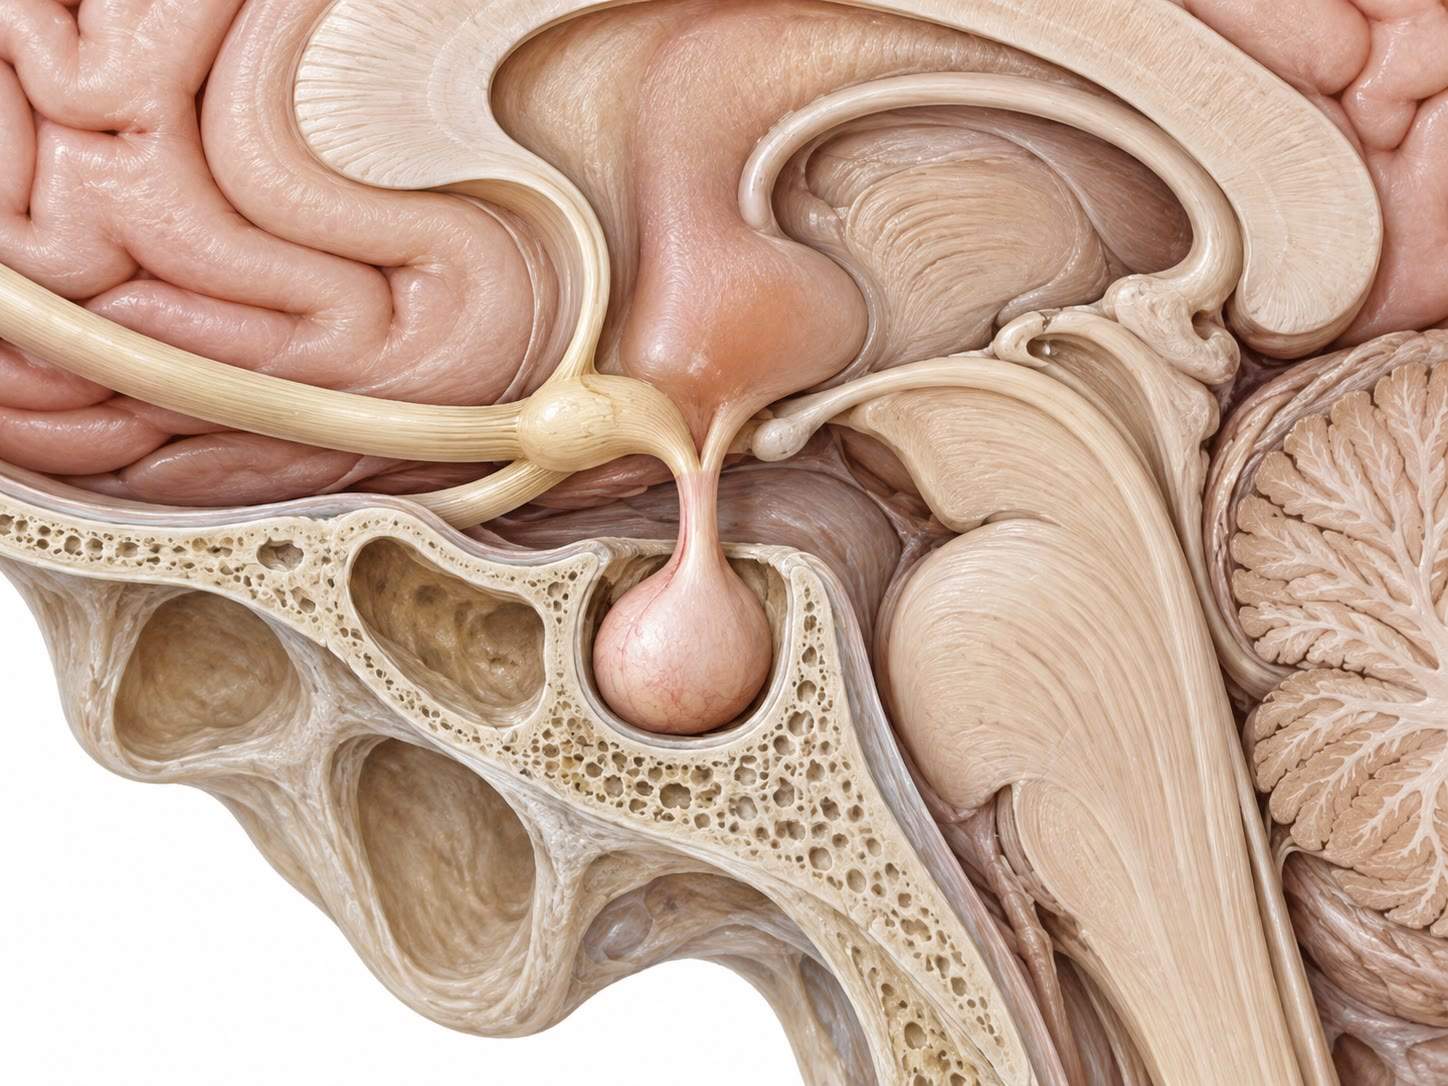
\includegraphics[width=0.55\linewidth]{images/book4/ai/b4-09-hypothalamus-pituitary.jpg}

{\small A base do encéfalo em corte sagital: o hipotálamo acima, a
haste e a hipófise em sua cavidade óssea --- o equipamento material do
eixo.}
\end{omfigure}

\section{O homem: controle tônico}

\begin{proposition}[O controle do testículo]\label{prop:b2:reproductive-hormones:testis}
\index{testosterona}\index{inibina}
O LH age sobre as \omterm{def:b2:mammal-reproduction:testis}{células de Leydig}, que produzem \emph{testosterona}
(\qtyrange{3}{10}{ng/mL} no sangue de um homem adulto, cem vezes mais
dentro do \omterm{def:b2:mammal-reproduction:testis}{testículo}). O FSH age sobre as \omterm{def:b2:mammal-reproduction:testis}{células de Sertoli}, que ---
com a testosterona local --- sustentam a \omterm{def:b2:mammal-reproduction:testis}{espermatogênese} e secretam
\emph{inibina}. A testosterona exerce retroalimentação sobre o
hipotálamo e a hipófise, mantendo o LH baixo; a inibina exerce
retroalimentação sobre a hipófise, mantendo o FSH baixo. As duas alças
são \emph{negativas} e o sistema é \emph{tônico}: os níveis hormonais
flutuam com os pulsos e com o dia (mais altos pela manhã), mas não são
cíclicos, e os espermatozoides são produzidos continuamente. A
testosterona também constrói e mantém as glândulas acessórias e os
ductos, a barba, a voz, os músculos e os ossos, a produção de hemácias
e a libido, e no feto formou o corpo masculino (\cref{ch:b2:mammal-reproduction}). A castração
a elimina: o LH e o FSH sobem várias vezes por falta de
retroalimentação, e os caracteres secundários regridem; a testosterona
injetada restaura os caracteres --- mas não a fertilidade, porque ela
também suprime o LH e, portanto, a testosterona intratesticular de que
a \omterm{def:b2:mammal-reproduction:testis}{espermatogênese} necessita. É por isso que os esteroides anabolizantes
tornam os homens inférteis.
\end{proposition}
\begin{proof}[Evidências]
Berthold (1849) castrou frangos: suas cristas encolheram e eles
deixaram de cantar e de brigar. Um \omterm{def:b2:mammal-reproduction:testis}{testículo} enxertado no abdome de um
castrado, onde desenvolveu uma nova irrigação sanguínea mas nenhum
nervo, restaurou a crista, o canto e a briga: o \omterm{def:b2:mammal-reproduction:testis}{testículo} agia pelo
sangue --- a primeira demonstração de uma secreção interna, cinquenta
anos antes da palavra hormônio. A testosterona foi isolada e
sintetizada em 1935.
\end{proof}

\section{A mulher: um ciclo com uma chave}

\begin{definition}[Os ciclos ovariano e uterino]\label{def:b2:reproductive-hormones:cycle}
\index{ciclo menstrual}\index{fase folicular}\index{fase lútea}\index{pico de LH}\index{endométrio}
O ciclo é contado a partir do primeiro dia da menstruação e dura cerca
de 28 dias. \emph{Fase folicular} (dias 1--14): o FSH, livre da
retroalimentação pela morte do \omterm{def:b2:mammal-reproduction:ovary}{corpo lúteo} anterior, recruta uma
coorte de \omterm{def:b2:mammal-reproduction:ovary}{folículos}; estes secretam \emph{estradiol}, que sobe
continuamente; o estradiol e a inibina reduzem o FSH, e só o \omterm{def:b2:mammal-reproduction:ovary}{folículo}
com mais receptores de FSH sobrevive à queda --- o \omterm{def:b2:mammal-reproduction:ovary}{folículo} dominante.
No útero, o estradiol reconstrói o \emph{endométrio} (a fase
proliferativa) e torna o muco cervical mais fluido. \emph{\omterm{def:b2:mammal-reproduction:ovary}{Ovulação}}
(dia 14): quando o estradiol permanece acima de cerca de
\qty{200}{pg/mL} durante um dia e meio, sua retroalimentação sobre o
hipotálamo e a hipófise passa de negativa a \emph{positiva}; o LH sobe
dez vezes num dia --- o \emph{pico de LH} --- e cerca de 36 horas após
seu início o \omterm{def:b2:mammal-reproduction:ovary}{folículo} se rompe e libera o ovócito. \emph{Fase lútea}
(dias 15--28): o \omterm{def:b2:mammal-reproduction:ovary}{folículo} esvaziado se torna o \omterm{def:b2:mammal-reproduction:ovary}{corpo lúteo}, que, sob o
LH, secreta \emph{progesterona} (\qtyrange{10}{20}{ng/mL}) e estradiol;
a progesterona torna o endométrio secretor, espessa o muco, eleva a
temperatura corporal basal em \qty{0.3}{\celsius} e, com o estradiol,
suprime o LH e o FSH. O \omterm{def:b2:mammal-reproduction:ovary}{corpo lúteo} tem uma vida de cerca de 14 dias;
a menos que a hCG de um embrião o resgate, ele regride, a progesterona
e o estradiol caem, o endométrio descama (\emph{menstruação}), o FSH
sobe e o ciclo seguinte começa. A fase lútea é fixa, de 14 dias; a
variação da duração do ciclo é variação da fase folicular.
\end{definition}

\begin{omfigure}
\begin{tikzpicture}
\begin{axis}[
  width=0.94\linewidth, height=6.4cm,
  axis x line=bottom, axis y line=left,
  xmin=0, xmax=28, ymin=0, ymax=1.15,
  xlabel={dia do ciclo}, ylabel={hormônios (em relação ao pico)},
  xlabel style={font=\small, at={(axis description cs:0.5,-0.11)}, anchor=north},
  ylabel style={font=\small},
  tick label style={font=\small}, xtick={0,7,14,21,28}, ytick={0,0.5,1},
  legend style={font=\scriptsize, at={(0.5,-0.25)}, anchor=north, draw=none, legend columns=4},
  clip=false,
]
\addplot[very thick, omThm, domain=0:28, samples=120] {0.1 + 0.9*exp(-((x-14)^2)/0.9)};
\addlegendentry{LH}
\addplot[very thick, omProp, domain=0:28, samples=120] {0.35*exp(-x/6) + 0.15 + 0.35*exp(-((x-14)^2)/1.2)};
\addlegendentry{FSH}
\addplot[very thick, omDef, domain=0:28, samples=160] {0.1 + 0.9*exp(-((x-12.5)^2)/6) + 0.4*exp(-((x-21)^2)/12)};
\addlegendentry{estradiol}
\addplot[very thick, omExo!70!black, domain=0:28, samples=160] {0.03 + 0.97*exp(-((x-21)^2)/12)*(x>14)};
\addlegendentry{progesterona}
\draw[dashed, gray] (axis cs:14.5,0) -- (axis cs:14.5,1.1); \node[font=\scriptsize, anchor=south] at (axis cs:14.5,1.1) {ovulação};
\node[font=\scriptsize, anchor=north] at (axis cs:7,1.1) {fase folicular};
\node[font=\scriptsize, anchor=north] at (axis cs:21.5,1.1) {fase lútea};
\end{axis}
\end{tikzpicture}

{\small Os hormônios do ciclo. O estradiol do \omterm{def:b2:mammal-reproduction:ovary}{folículo} em crescimento
sobe ao longo da \omterm{def:b2:reproductive-hormones:cycle}{fase folicular} e, acima de um limiar, desencadeia o
\omterm{def:b2:reproductive-hormones:cycle}{pico de LH}; a \omterm{def:b2:mammal-reproduction:ovary}{ovulação} ocorre cerca de 36 horas depois; o \omterm{def:b2:mammal-reproduction:ovary}{corpo lúteo}
secreta então progesterona durante duas semanas e morre.}
\end{omfigure}

\begin{omfigure}
\begin{tikzpicture}[every node/.style={font=\scriptsize}]
  % endometrium thickness over the cycle
  \draw[thick, ->] (0,0) -- (12.4,0) node[right] {dia};
  \foreach \x/\l in {0/1, 2.1/5, 6.0/14, 12/28} \draw (\x,0.08) -- (\x,-0.08) node[below] {\l};
  \fill[omThm!25] (0,0) -- (0,1.4) .. controls (0.8,1.2) and (1.6,0.5) .. (2.1,0.35) -- (2.1,0) -- cycle;
  \fill[omDef!20] (2.1,0) -- (2.1,0.35) .. controls (3.5,0.6) and (5.2,1.3) .. (6.0,1.5) -- (6.0,0) -- cycle;
  \fill[omExo!35] (6.0,0) -- (6.0,1.5) .. controls (8,1.8) and (11,1.9) .. (12,1.6) -- (12,0) -- cycle;
  \node at (1.0,1.8) {menstruação};
  \node at (4.0,1.8) {proliferativa (estradiol)};
  \node at (9,2.2) {secretora (progesterona): glândulas, glicogênio, artérias espiraladas};
  \node[anchor=east] at (-0.1,0.8) {endométrio};
\end{tikzpicture}

{\small O ciclo uterino. O \omterm{def:b2:reproductive-hormones:cycle}{endométrio} descama na menstruação, é
reconstruído sob o estradiol e se torna secretor sob a progesterona,
pronto para receber um \omterm{def:b2:mammal-reproduction:implantation}{blastocisto} por volta do dia 21; quando a
progesterona cai, ele descama de novo.}
\end{omfigure}

\begin{omfigure}
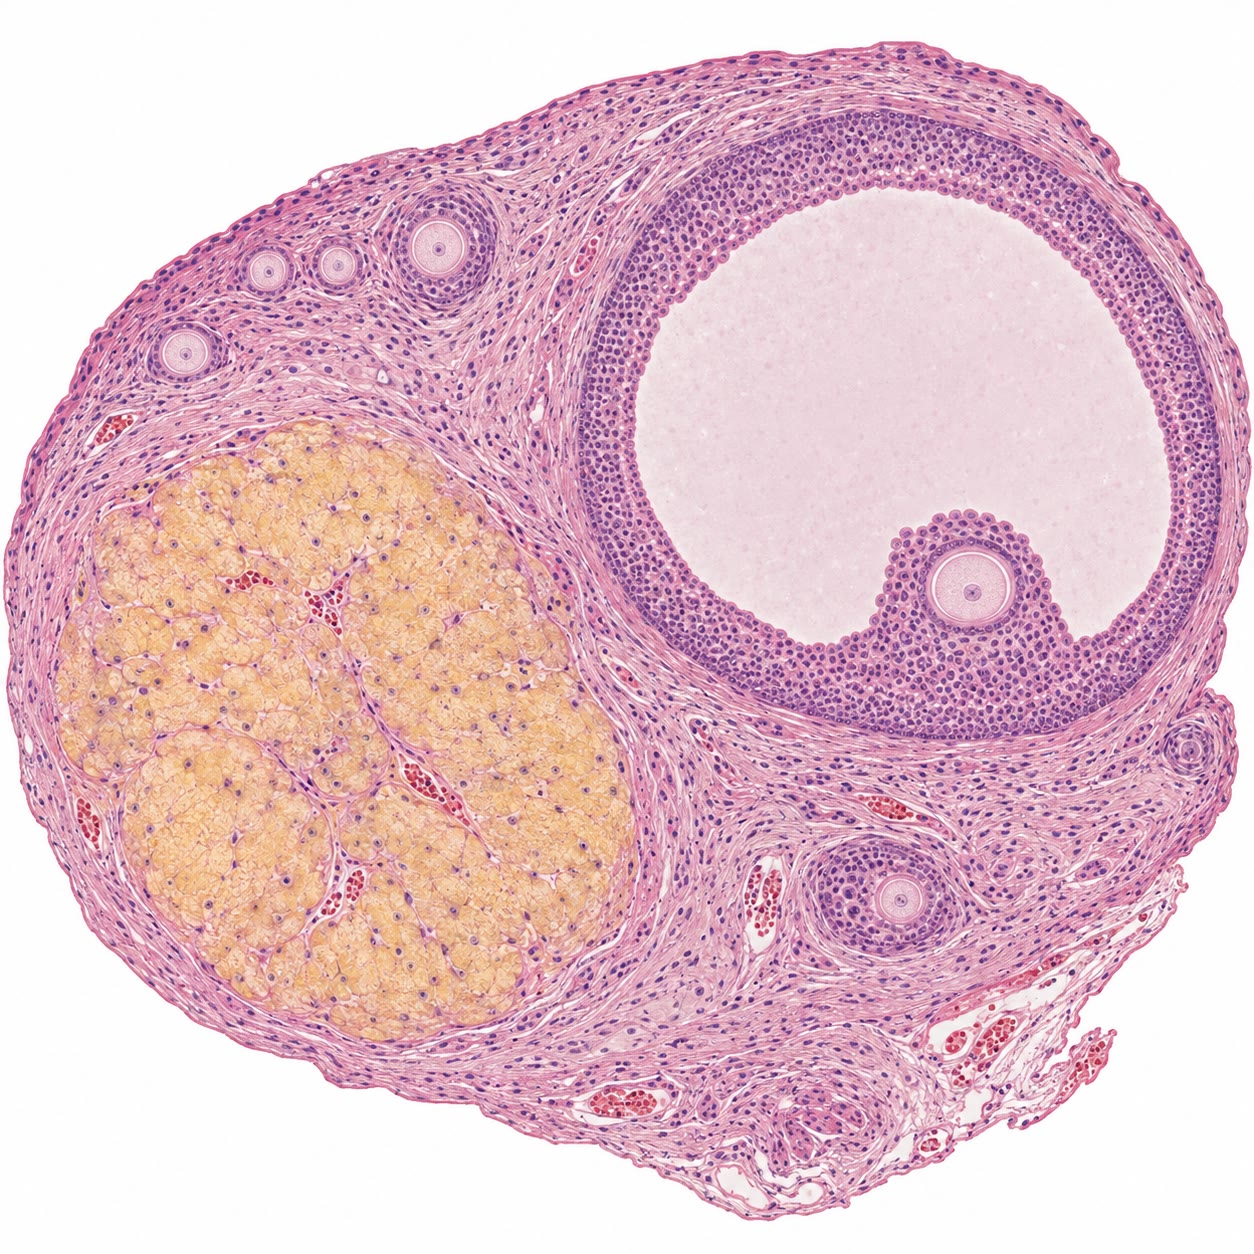
\includegraphics[width=0.46\linewidth]{images/book4/ai/b4-09-ovary-histology.jpg}

{\small Um ovário em corte: um \omterm{def:b2:mammal-reproduction:ovary}{folículo} maduro com sua cavidade e seu
ovócito, pequenos \omterm{def:b2:mammal-reproduction:ovary}{folículos} primordiais sob a superfície e um \omterm{def:b2:mammal-reproduction:ovary}{corpo
lúteo} de um ciclo anterior.}
\end{omfigure}

\begin{theorem}[A passagem da retroalimentação negativa à positiva]\label{thm:b2:reproductive-hormones:switch}
\index{retroalimentação positiva!pico de LH}
O estradiol, nos níveis baixos do início da \omterm{def:b2:reproductive-hormones:cycle}{fase folicular}, inibe o LH
e o FSH; o estradiol acima de cerca de \qty{200}{pg/mL}, mantido por
mais de cerca de \qty{36}{h}, faz o contrário: leva o hipotálamo a
liberar uma descarga de GnRH e a hipófise a responder com um aumento
de dez vezes do LH. O mecanismo é uma mudança de sinal, e não de
magnitude: uma dose alta e sustentada induz na hipófise um grande
estoque de LH e uma sensibilidade aumentada ao GnRH, e no hipotálamo
(por meio dos neurônios de kisspeptina) a passagem do gerador de pulsos
de GnRH a um modo de pico. A chave converte um sinal graduado --- a
quantidade de estradiol que o \omterm{def:b2:mammal-reproduction:ovary}{folículo} produz --- num evento de tudo ou
nada sincronizado no dia, que é o que a \omterm{def:b2:mammal-reproduction:ovary}{ovulação} exige; e, como só um
\omterm{def:b2:mammal-reproduction:ovary}{folículo} grande e maduro consegue sustentar \qty{200}{pg/mL}, o pico
só dispara quando há um óvulo pronto para ser liberado. Uma vez
ocorrida a \omterm{def:b2:mammal-reproduction:ovary}{ovulação}, a progesterona do \omterm{def:b2:mammal-reproduction:ovary}{corpo lúteo} restabelece a
retroalimentação negativa, e nenhum segundo pico se segue.
\end{theorem}
\begin{proof}[Evidências]
Em mulheres e macacas com o eixo suprimido, uma infusão de estradiol
que eleva o nível plasmático acima de \qty{200}{pg/mL} durante dois
dias é seguida de um \omterm{def:b2:reproductive-hormones:cycle}{pico de LH}; a mesma quantidade administrada
durante um dia, ou um nível mais baixo durante três, não o é. A
progesterona administrada antes da infusão bloqueia o pico;
administrada ao mesmo tempo, o antecipa e o amplifica. O limiar em
dose e em duração reproduz o momento do pico natural a partir da
subida natural do estradiol.
\end{proof}

\section{Sobrepujar o ciclo}

\begin{proposition}[Gestação, lactação, menopausa]\label{prop:b2:reproductive-hormones:overrides}
\index{gonadotrofina coriônica humana}\index{menopausa}
Um embrião em \omterm{def:b2:mammal-reproduction:implantation}{implantação} secreta \emph{hCG}, um hormônio semelhante ao
LH que se liga ao receptor de LH e mantém o \omterm{def:b2:mammal-reproduction:ovary}{corpo lúteo} vivo e
secretando além de seus quatorze dias; na semana dez, a própria
\omterm{def:b2:mammal-reproduction:placenta}{placenta} produz progesterona e estrógenos suficientes para manter a
gestação, e o \omterm{def:b2:mammal-reproduction:ovary}{corpo lúteo} se torna dispensável. Durante toda a
gestação, os esteroides elevados mantêm o LH e o FSH em zero: nenhum
\omterm{def:b2:mammal-reproduction:ovary}{folículo} cresce, nenhuma \omterm{def:b2:mammal-reproduction:ovary}{ovulação} ocorre. Após o nascimento, a sucção
eleva a prolactina e desacelera os pulsos de GnRH, e a \omterm{def:b2:mammal-reproduction:ovary}{ovulação}
permanece suprimida durante meses. Na \emph{menopausa}, o estoque de
\omterm{def:b2:mammal-reproduction:ovary}{folículos} se esgota: o estradiol e a inibina caem e, sem nada que
exerça retroalimentação, o LH e o FSH sobem a dez vezes seu nível
anterior e ali permanecem --- a assinatura de uma glândula que deixou
de responder.
\end{proposition}

\begin{proposition}[Contracepção e reprodução assistida]\label{prop:b2:reproductive-hormones:clinic}
\index{contracepção!hormonal}\index{fecundação in vitro}
A pílula combinada fornece todos os dias um estrógeno sintético e um
progestagênio: o nível constante de esteroides mantém o FSH e o LH
baixos, nenhum \omterm{def:b2:mammal-reproduction:ovary}{folículo} é recrutado, nenhuma subida de estradiol
ocorre e o pico nunca dispara; o progestagênio também espessa o muco
cervical. A pausa de sete dias deixa o \omterm{def:b2:reproductive-hormones:cycle}{endométrio} sangrar; esquecer
comprimidos por mais de dois dias seguidos permite que o FSH escape e
um \omterm{def:b2:mammal-reproduction:ovary}{folículo} pode crescer. A contracepção de emergência adia o pico por
alguns dias com uma dose alta de progestagênio. Na \emph{\omterm{prop:b2:reproductive-hormones:clinic}{fecundação in
vitro}}, o eixo é conduzido no sentido oposto: FSH diário durante dez
dias sobrepuja a seleção de um único \omterm{def:b2:mammal-reproduction:ovary}{folículo} dominante e faz
amadurecer dez ou mais; um antagonista de GnRH impede um pico
espontâneo prematuro; uma injeção de hCG substitui o pico, e os
ovócitos são coletados 34 a 36 horas depois, pouco antes de serem
liberados; eles são fecundados na placa, e um ou dois embriões são
transferidos, sendo os demais congelados. No homem, a testosterona
exógena ou um análogo de GnRH suprime a \omterm{def:b2:mammal-reproduction:testis}{espermatogênese} ao suprimir o
LH --- o princípio de um contraceptivo hormonal masculino, ainda não
comercializado. Tudo isso é o eixo da primeira seção, lido de trás
para a frente.
\end{proposition}

\section{Exercícios}

\begin{exercise}[$\star$]\label{exo:b2:reproductive-hormones:1}
Desenhe o eixo no homem: os três níveis, os quatro hormônios, as duas
alças de retroalimentação e as células sobre as quais cada hormônio
age.
\end{exercise}

\begin{exercise}[$\star$]\label{exo:b2:reproductive-hormones:2}
Dê as fases dos ciclos ovariano e uterino, com seus dias e o hormônio
que domina cada uma.
\end{exercise}

\begin{exercise}[$\star$]\label{exo:b2:reproductive-hormones:3}
Explique como a pílula combinada impede a \omterm{def:b2:mammal-reproduction:ovary}{ovulação}, e por que ocorre
sangramento na semana sem pílula.
\end{exercise}

\begin{exercise}[$\star$]\label{exo:b2:reproductive-hormones:4}
O que acontece com o LH, o FSH e os caracteres sexuais secundários de
um homem adulto castrado? Quais desses efeitos a testosterona injetada
reverte, e quais não?
\end{exercise}

\begin{exercise}[$\star\star$]\label{exo:b2:reproductive-hormones:5}
Os pulsos de GnRH ocorrem a cada \qty{90}{min} na \omterm{def:b2:reproductive-hormones:cycle}{fase folicular} e a
cada \qty{4}{h} na \omterm{def:b2:reproductive-hormones:cycle}{fase lútea}. Quantos pulsos por dia em cada uma? A
hipófise favorece o LH com pulsos rápidos e o FSH com pulsos lentos:
que gonadotrofina deve subir primeiro quando o \omterm{def:b2:mammal-reproduction:ovary}{corpo lúteo} morre, e
por que é a gonadotrofina certa?
\end{exercise}

\begin{exercise}[$\star\star$]\label{exo:b2:reproductive-hormones:6}
Converta \qty{200}{pg/mL} de estradiol (massa molar
\qty{272}{g/mol}) em \unit{pmol/L}, e \qty{15}{ng/mL} de
progesterona (\qty{314}{g/mol}) em \unit{nmol/L}. Quantas moléculas
de estradiol há num microlitro de plasma no limiar do pico?
\end{exercise}

\begin{exercise}[$\star\star$]\label{exo:b2:reproductive-hormones:7}
Os ciclos de uma mulher duram 35 dias. Sabendo que a \omterm{def:b2:reproductive-hormones:cycle}{fase lútea} é
fixa, em que dia ela ovula, e quais dias são férteis se os
espermatozoides sobrevivem três dias e o óvulo um? Por que o método do
calendário falha para ciclos irregulares?
\end{exercise}

\begin{exercise}[$\star\star$]\label{exo:b2:reproductive-hormones:8}
Um embrião se implanta no dia 21 de um ciclo de 28 dias, e sua hCG,
partindo de \qty{1}{UI/L}, dobra a cada dois dias. O \omterm{def:b2:mammal-reproduction:ovary}{corpo lúteo}
precisa de algumas UI/L de hCG até o dia 26 para sobreviver. O embrião
chega a tempo? O que aconteceria se a \omterm{def:b2:mammal-reproduction:implantation}{implantação} fosse adiada para o
dia 25?
\end{exercise}

\begin{exercise}[$\star\star$]\label{exo:b2:reproductive-hormones:9}
Diga o que o experimento de Knobil mostrou e o que ele descartou, e
preveja o efeito de administrar a uma mulher um agonista de GnRH de
ação prolongada durante um mês: sobre o LH, sobre o estradiol, sobre o
\omterm{def:b2:reproductive-hormones:cycle}{endométrio}.
\end{exercise}

\begin{exercise}[$\star\star\star$]\label{exo:b2:reproductive-hormones:10}
No modelo dos receptores, tome $s = 100$ receptores por hora, $d =
\qty{0.5}{h^{-1}}$ e $iH = \qty{6}{h^{-1}}$ enquanto houver hormônio.
Calcule o número estacionário de receptores sem hormônio e com hormônio
contínuo. Com um pulso de dois minutos a cada hora, calcule o número
perdido por pulso e a fração do déficit recuperada antes do pulso
seguinte, e deduza o nível em torno do qual o estoque se estabiliza.
\end{exercise}

\begin{exercise}[$\star\star\star$]\label{exo:b2:reproductive-hormones:11}
Uma mulher na pós-menopausa tem LH e FSH dez vezes acima do nível de
uma mulher jovem e estradiol muito baixo; uma mulher com um tumor
hipofisário secretor de prolactina tem LH baixo, estradiol baixo e
nenhum ciclo; uma mulher com um tumor de células da granulosa tem
estradiol alto, LH baixo e nenhum ciclo. Explique cada perfil a partir
do eixo.
\end{exercise}

\begin{exercise}[$\star\star\star$]\label{exo:b2:reproductive-hormones:12}
``O mesmo hormônio inibe e depois desencadeia o \omterm{def:b2:reproductive-hormones:cycle}{pico de LH}.'' Explique
como o estradiol pode ter os dois efeitos, por que a \omterm{def:b2:mammal-reproduction:ovary}{ovulação} precisa
de uma chave e não de um regulador gradual, e o que daria errado com um
regulador gradual.
\end{exercise}

\section{Problema: Um ciclo medido}

\begin{problem}[{Problema de fim de semana --- dosagens hormonais
diárias de um ciclo são lidas para identificar as fases, o dia da
ovulação e a janela fértil; o limiar do pico, o relógio do corpo lúteo
e o resgate pela hCG são calculados; o modelo dos receptores explica
Knobil; e o eixo é conduzido no sentido inverso na clínica, até o dia
da ovulação, a duração da fase lútea, a janela fértil e o limiar do
pico}]
\label{pb:b2:reproductive-hormones:1}
Colheu-se sangue em dias selecionados do ciclo de uma mulher:

\begin{center}
\small
\begin{tabular}{lcccccccccc}
\hline
dia & 1 & 5 & 8 & 11 & 12 & 13 & 14 & 15 & 21 & 27 \\
\hline
estradiol (\unit{pg/mL}) & 40 & 60 & 110 & 210 & 260 & 310 & 220 & 150 & 160 & 50 \\
LH (\unit{UI/L}) & 5 & 5 & 6 & 7 & 8 & 20 & 65 & 15 & 4 & 4 \\
progesterona (\unit{ng/mL}) & 0.5 & 0.5 & 0.6 & 0.7 & 0.8 & 1.0 & 1.5 & 3 & 16 & 2 \\
temperatura (\unit{\celsius}) & 36.4 & 36.4 & 36.4 & 36.4 & 36.4 & 36.4 & 36.4 & 36.5 & 36.8 & 36.7 \\
\hline
\end{tabular}
\end{center}

A menstruação começou no dia 1 e de novo no dia 29.

\medskip
\noindent\textbf{Parte I --- A leitura do ciclo.}
\begin{enumerate}
  \item Identifique as \omterm{def:b2:reproductive-hormones:cycle}{fases folicular} e lútea a partir da tabela, com
        o hormônio que marca cada uma.
  \item Em que dia o \omterm{def:b2:reproductive-hormones:cycle}{pico de LH} atingiu o máximo? Quando ocorreu a
        \omterm{def:b2:mammal-reproduction:ovary}{ovulação}?
  \item Quanto durou a \omterm{def:b2:reproductive-hormones:cycle}{fase lútea}? Isso é coerente com a vida do \omterm{def:b2:mammal-reproduction:ovary}{corpo
        lúteo}?
  \item Explique a mudança de temperatura e por que ela confirma, mas
        não consegue prever, a \omterm{def:b2:mammal-reproduction:ovary}{ovulação}.
  \item Em que dias o estradiol esteve acima de \qty{200}{pg/mL}?
        Relacione essa duração com o pico.
  \item Dê a janela fértil desse ciclo (espermatozoides três dias,
        óvulo um dia).
\end{enumerate}

\medskip
\noindent\textbf{Parte II --- Números.}
\begin{enumerate}[resume]
  \item Converta o estradiol do dia 13 em \unit{pmol/L}, e a
        progesterona do dia 21 em \unit{nmol/L}.
  \item Por que fator o LH subiu do dia 12 ao dia 14? Por que ele cai
        tão depressa depois (a meia-vida do LH é de cerca de
        \qty{1}{h})?
  \item Se o ciclo seguinte dessa mulher tivesse uma \omterm{def:b2:reproductive-hormones:cycle}{fase folicular} de
        21 dias, em que dia ela ovularia e qual seria a duração do
        ciclo?
  \item Um embrião se implanta 7 dias após a \omterm{def:b2:mammal-reproduction:ovary}{ovulação}. Em que dia desse
        ciclo a hCG apareceria e, dobrando a cada dois dias a partir de
        \qty{1}{UI/L}, que nível atingiria no dia 27?
  \item Explique por que a progesterona de \qty{2}{ng/mL} no dia 27
        mostra que nenhum embrião se implantou.
  \item Quais teriam sido os valores de progesterona e de estradiol no
        dia 27 se um embrião tivesse se implantado?
\end{enumerate}

\medskip
\noindent\textbf{Parte III --- Retroalimentação e pulsos.}
\begin{enumerate}[resume]
  \item Explique, com os sinais das retroalimentações, por que o FSH é
        mais alto no início do ciclo e por que normalmente só um
        \omterm{def:b2:mammal-reproduction:ovary}{folículo} sobrevive.
  \item No modelo dos receptores com $s = 100$ por hora, $d =
        \qty{0.5}{h^{-1}}$, $iH = \qty{6}{h^{-1}}$, calcule $R^*$ sem
        hormônio e sob hormônio contínuo.
  \item Um pulso dura \qty{2}{min}. Partindo do $R^*$ sem estímulo,
        quantos receptores um pulso remove (use a aproximação linear
        $iHR\,\Delta t$)? Que fração do déficit é recuperada na hora
        anterior ao pulso seguinte (constante de tempo $1/d$), e em
        torno de que nível o estoque se estabiliza?
  \item Use esses números para explicar o resultado de Knobil.
  \item Um homem recebe continuamente um agonista de GnRH para um
        câncer de próstata. Preveja seu LH e sua testosterona após um
        dia e após um mês, e explique a diferença.
  \item As células da granulosa de uma mulher não produzem inibina.
        Preveja seu FSH e seu LH, e a consequência para o recrutamento
        dos \omterm{def:b2:mammal-reproduction:ovary}{folículos}.
\end{enumerate}

\medskip
\noindent\textbf{Parte IV --- A clínica.}
\begin{enumerate}[resume]
  \item Para uma \omterm{prop:b2:reproductive-hormones:clinic}{fecundação in vitro}, essa mulher recebe FSH
        diariamente a partir do dia 2. Explique por que dez \omterm{def:b2:mammal-reproduction:ovary}{folículos}
        amadurecem em vez de um.
  \item Por que se acrescenta um antagonista de GnRH a partir do dia 6,
        e o que aconteceria sem ele?
  \item A hCG é injetada quando os \omterm{def:b2:mammal-reproduction:ovary}{folículos} estão maduros; os ovócitos
        são coletados 35 horas depois. Justifique esse momento a partir
        da tabela.
  \item Dez ovócitos são coletados; \qty{70}{\%} são fecundados,
        \qty{40}{\%} dos embriões chegam ao estágio de \omterm{def:b2:mammal-reproduction:implantation}{blastocisto}, e
        cada \omterm{def:b2:mammal-reproduction:implantation}{blastocisto} transferido se implanta com probabilidade
        $0.35$. Número esperado de \omterm{def:b2:mammal-reproduction:implantation}{blastocistos}? Probabilidade de pelo
        menos uma gravidez se dois forem transferidos?
  \item Explique por que a pílula combinada, tomada por essa mulher,
        teria produzido uma tabela sem \omterm{def:b2:reproductive-hormones:cycle}{pico de LH} e sem subida da
        progesterona.
  \item Um contraceptivo masculino baseado num antagonista de GnRH
        também eliminaria a testosterona. O que é preciso administrar
        junto, e por que isso não restaura a produção de
        espermatozoides?
  \item Enuncie o resultado: dia da \omterm{def:b2:mammal-reproduction:ovary}{ovulação}, duração da \omterm{def:b2:reproductive-hormones:cycle}{fase lútea},
        janela fértil, e o limiar e a duração do estradiol que
        desencadearam o pico.
\end{enumerate}
\end{problem}
